\chapter{Boosted Physics as an Experimental Tool}
\label{ch:boost}

\section{The ``impossible'' Higgs decay}
The standard model Higgs boson couples to fermions according to their mass. With the heaviest fermion available for Higgs decay being the b quark, the 58\% of Higgs will decay to pairs of these quarks. The two leading discovery channels for the Higgs, however, were the \higgstoZZtollll and \higgstogammagamma gamma decays which make up less than half a percent of Higgs decays, far less frequent than a decay to b quarks \cite{pdg2018}. However, from the beginning of the design of \CMS and the LHC, it was not expected to be possible to even measure \higgstobb as the rate at which everyday QCD processes can produce pairs of b quarks is vastly higher than the Higgs process.

As the collision energy and luminosity of the \LHC increased in Run II, a possible new technique for analyzing Higgs decays emerged. Some small fraction of Higgs are produced in the \LHC with significant momentum. This Higgs momentum, or ``boost'', collimates the decay products of the Higgs in the lab frame making the signature distinct from a QCD process. A QCD process is very unlikely to produce two relatively collinear heavy quark pairs with significant momentum. While the chance of a boosted Higgs is also low, the ratio of signal to background rises dramatically with the requirement of a boosted object. The new challenge then, is distinguishing two individual b quarks pushed together into a single jet by the boost of the Higgs. For full details on the boosted \higgstobb analysis see \cite{boostedHiggsTobb}

The substructure of jets made in the merging of objects (including higher energy jets) is the subject of ongoing study at the \CMS and the \LHC. The ability to distinguish multiple objects within jets allowed \CMS to publish the groundbreaking measurement of the Higgs to bb decay in 2018. This thesis borrows some of these techniques to expand the mass limits on the \WR and \NR where the \NR forms a merged jet. These are discussed in the following sections.

\section{Boost}
Before delving too deeply into the algorithms used to study jet substructure, it's important to take a step back and cover the basics of boost as a special relativity concept and one of the more simple examples of it at \CMS, the decay of a boosted particle into two parts.
\subsection{Special Relativity}
Boost is a concept coming from special relativity. A basic premise of special relativity is that the speed of light should always be observed as constant, regardless of the relative motion of the observer with the respect to the emitter.
The consequences of this, time dilation and length contraction, are observed at the LHC as particles generally travel close to the speed of light. Distances parallel to the motion of the particles are measured shorter in the lab frame than they would be measured with the particles at rest. Both time dilation and length contraction are proportional to $\gamma$, which is called ``the boost''. The boost can be written as a function of the speed of an object and the speed of light, or in natural units is the ratio of the energy over the rest mass of a particle:

\begin{equation}
    \label{eq:lengthcontraction}
    \gamma
    =
    E / m_{0} .
\end{equation}
Using $\gamma$, the length contraction and time dilation can be defined as
\begin{equation}
    \label{eq:lengthandtime}
    L
    =
    L_{0} / \gamma ,
    \  
    t
    =
    \gamma t_{0} .
\end{equation}
 A measured proper length $L_0$, or the length measured when at rest, is divided by $\gamma$ and becomes equal to lab measured value. The proper time $t_0$ is dilated by the factor $\gamma$. However, distances perpendicular to the motion are not affected.

\subsection{Boosted Two-Body Decays}
The effect of special relativity only contracting the parallel coordinates can have significant effects on a process as viewed in the lab frame. As an example, consider a process like \higgstobb.  Considered at rest, the two decay quarks will travel back to back, to conserve momentum. As can often happen at the \LHC, the Higgs boson is produced with significant momentum, and while its decay particles are produced back-to-back in the Higgs frame of reference, they are additionally travelling in the direction of the Higgs in the lab frame. This results in two quarks which travel in the same direction in the lab frame.

\begin{figure}[!tp]
    \centering
    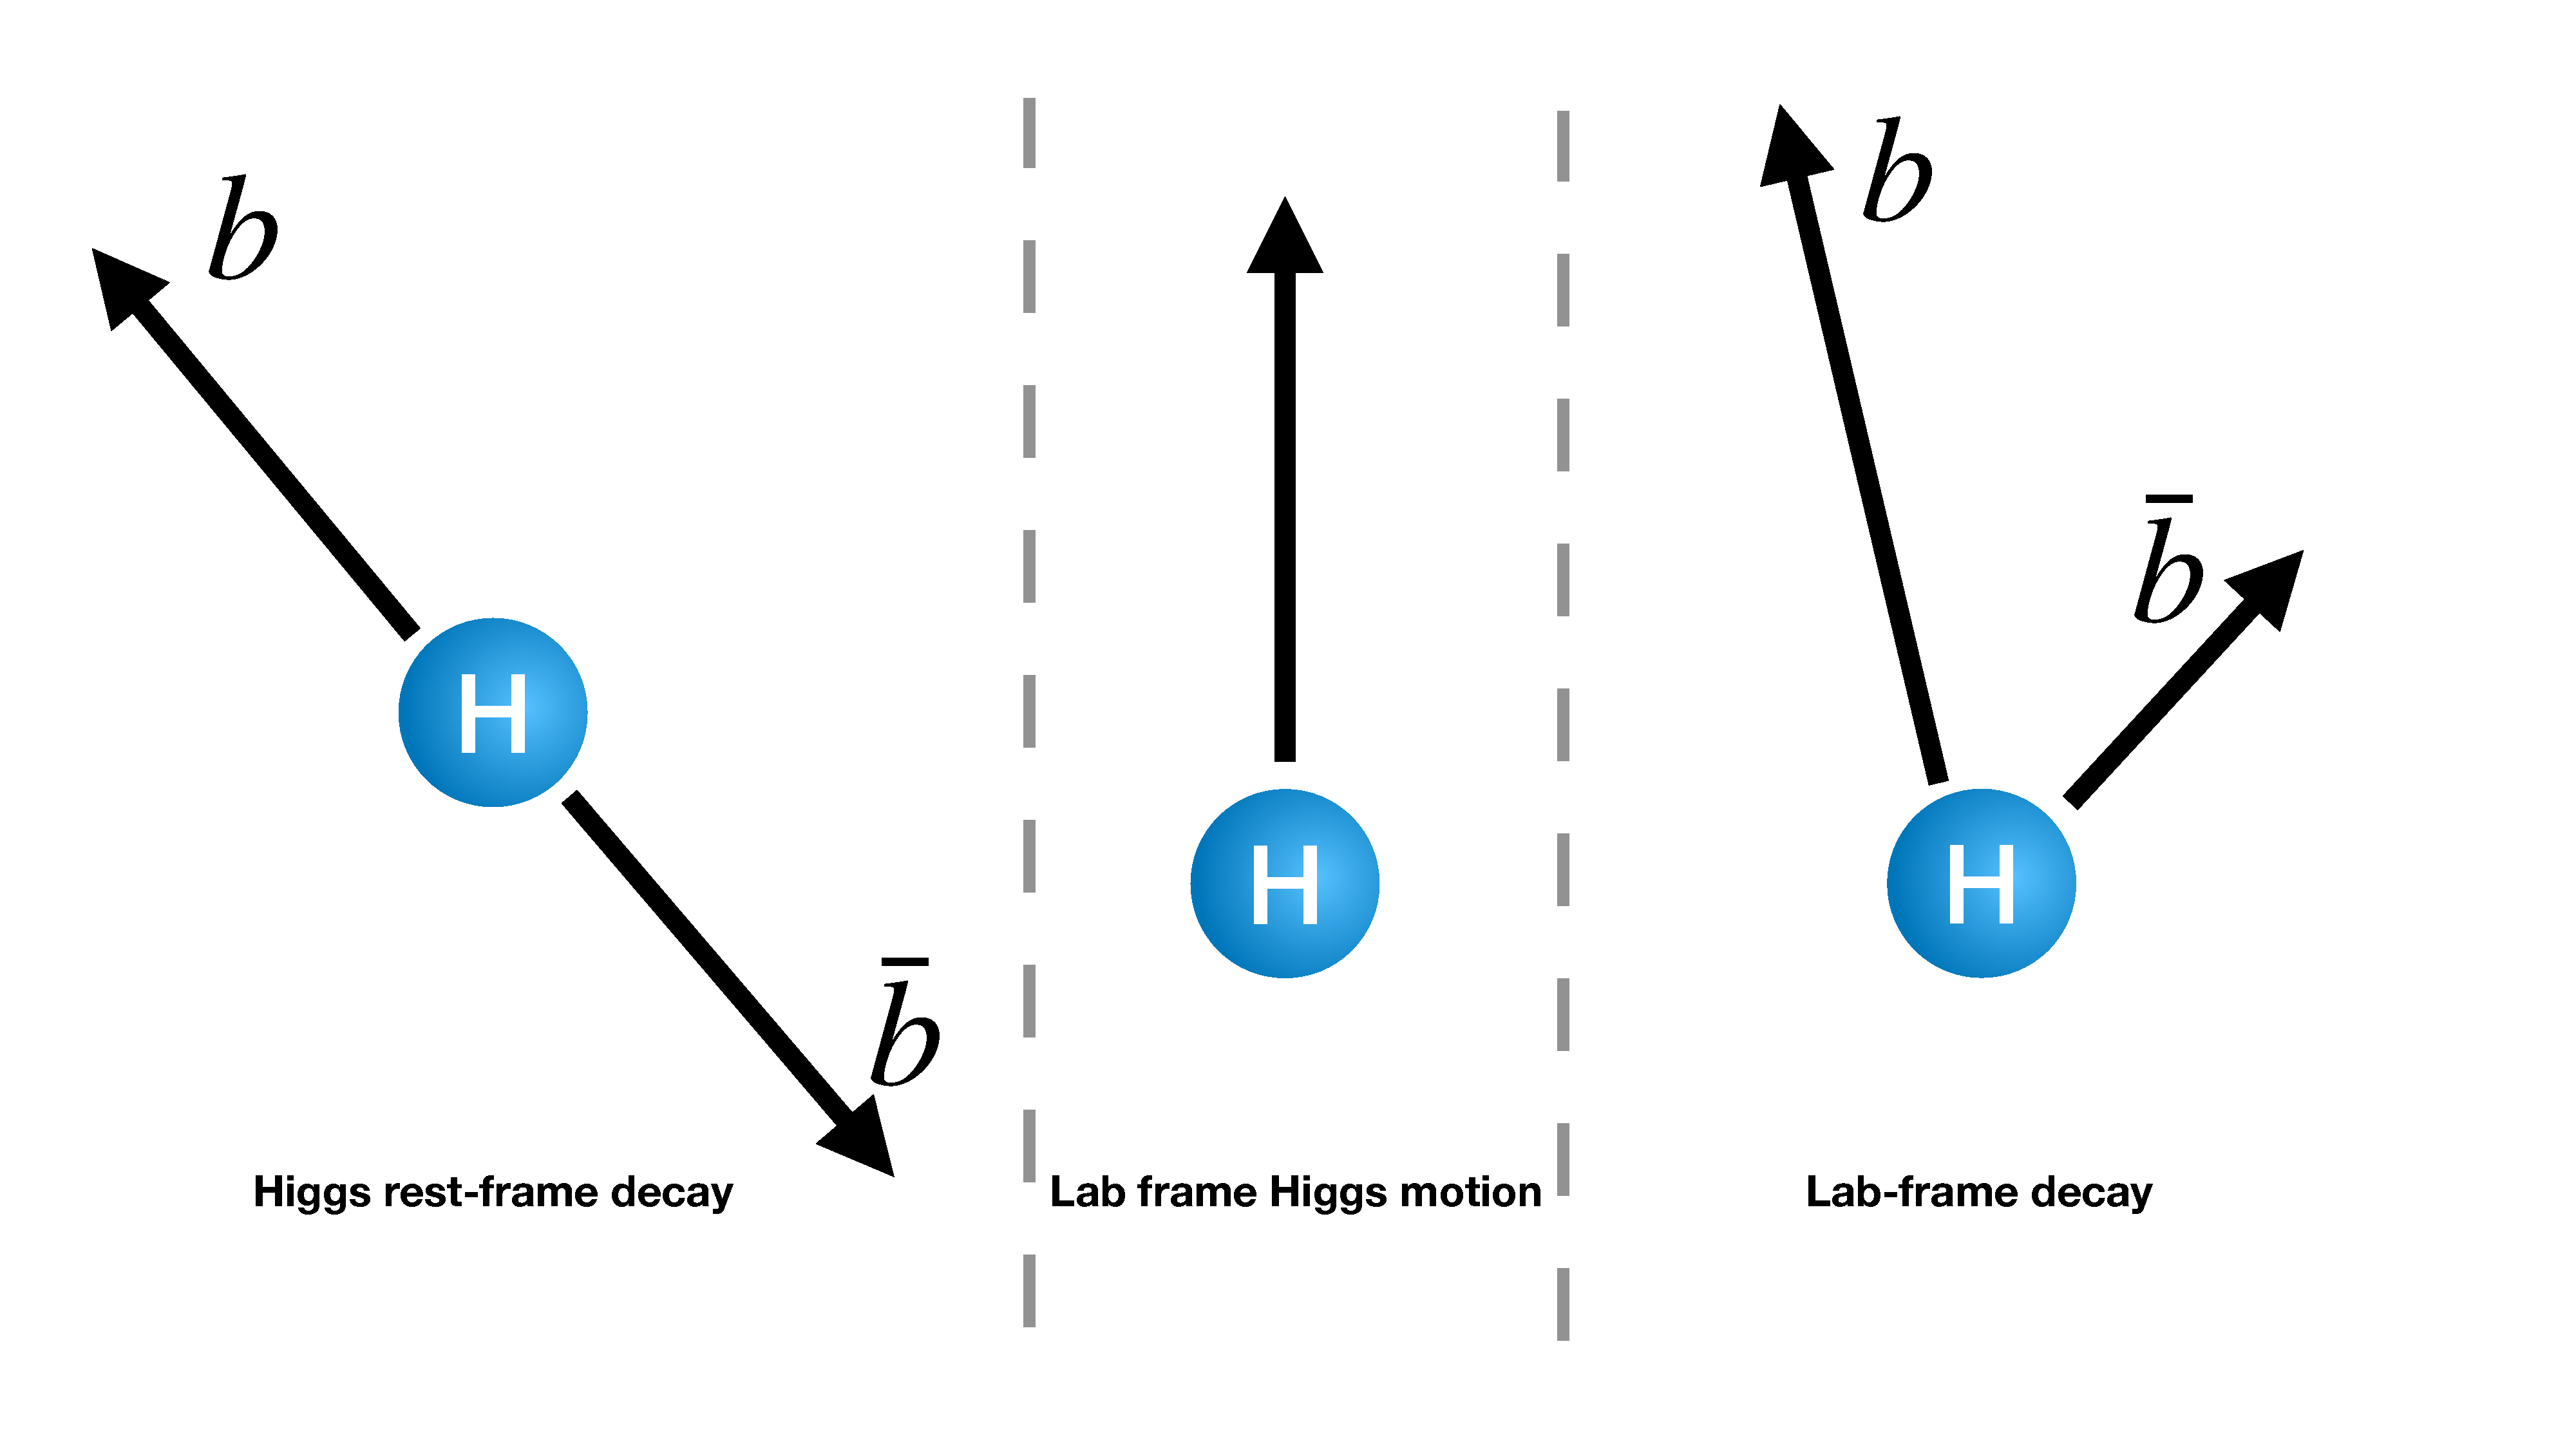
\includegraphics[width=\textwidth]{figures/twobodydecay.pdf}
    \caption[
        %short caption
        Boosted two-body Higgs boson decay
    ]    
    {
        On the left, a back-to-back decay of the Higgs to two b quarks is shown. With significant momentum of the Higgs, this process is observed differently in the lab frame of reference, shown on the right.
    }
    \label{fig:twobody}

\end{figure}

When the momentum of the particle undergoing decay is larger than its rest mass, the momentum the decay particles get from the boost will exceed the momentum received from the decay energy itself. In this case, and as is shown in Fig.~\ref{fig:twobody}, the decay particles will both travel in the direction of the initial particle, and in the lab frame appear closer and closer to each other as the boost continues to increase. At \CMS, a rule of thumb in a two body decay is that the angular separation between the particles proportional to the mass and transverse momentum of the initial particle:
\begin{equation}
    \label{eq:lengthandtime}
    \Delta R
    \approx
    2m / \pt .
\end{equation}

\section{Techniques in Boosted Physics at Hadron Colliders}

To leverage the kinematic uniqueness of boosted systems, including meson ones, significant advancements in techniques have arrived in recent years for the study of jets formed from particles seen as a merged together as a result of their boost.

\subsection{Jet Substructure}

Jet algorithms used in particle physics experiments like \CMS or \ATLAS are focused towards collecting all of the particles from a single quark or gluon.  There is, however, a significant amount of information that can be understood by looking at scales smaller than the size of jets reconstructed at \CMS. While a typical jet at \CMS is reconstructed with a size of \ensuremath{R_{cone} = 0.4 \| 0.8}, these jets can be re-clustered into smaller pieces.  A jet produced from a single quark may not have much interesting information at a finer scale, however, top quark jets, where multiple decays occur in-flight, or jets formed by the merger of multiple distinct objects may have interesting structural components.  Substructure analysis can also be used to decompose larger jets, like those used in this boosted analysis, which can contain several components. Several different techniques can be used look at the contents of jets.  N-subjettiness is used to determine how many subclusters a jet has, key for identification of jets in the boosted Higgs analysis. Those used in this analysis are lepton subjet fraction (LSF) and soft-drop mass and are discussed further below, as well as N-subjettiness which was studied but not used.

\subsubsection{N-subjettiness}

N-subjettiness was developed to be used to discriminate hadronically-decaying electro-weak bosons and top quarks from heavy QCD jets. N-subjettiness relies on the calculation of $\tau_{N}$ for different numbers of subjets, N.

\begin{equation}
    \label{eq:nsubjettiness}
    \tau_{N}
    =
    \frac{1}{d_{0}}\sum_{k} {p_{T,k} \mathrm{min} \left\{\Delta R_{1,k}, \Delta R_{2,k},\cdots,\Delta R_{N,k} \right\} } .
\end{equation}

The ratio of $\tau_{2}$ and $\tau_{1}$ is often used, but in principle any ratio can be used. This analysis studied the benefits of various N-subjettiness ratios, and did not find any to be particularly helpful for discriminating signal and background. A complete discussion of N-subjettiness is found in \cite{Nsubjettiness}.

\begin{figure}[!tp]
    \centering
    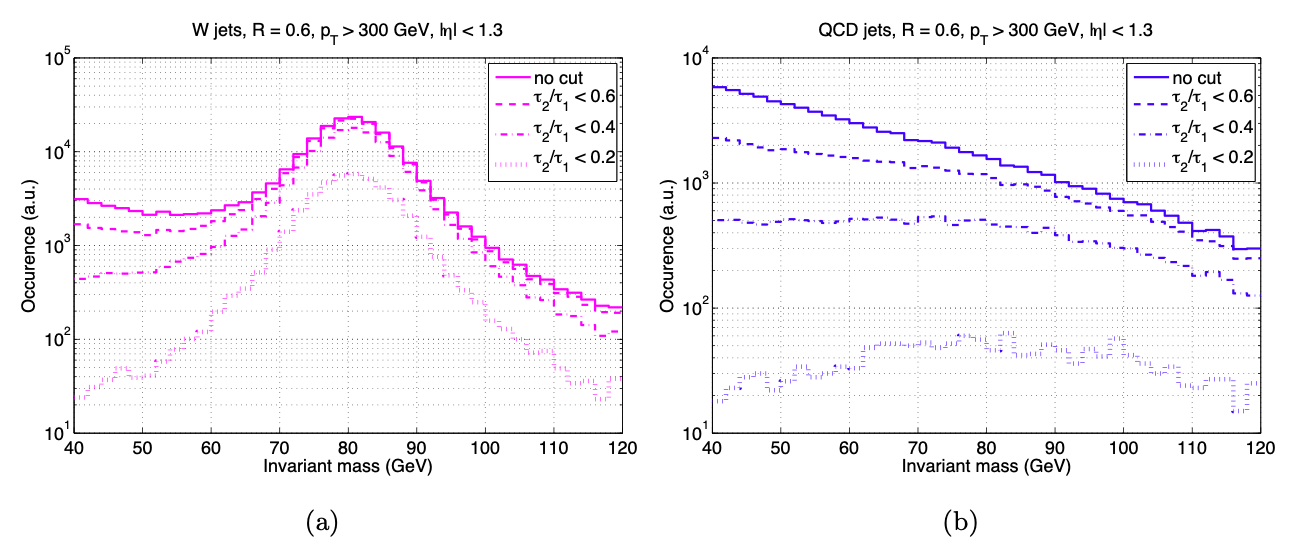
\includegraphics[width=\textwidth]{figures/Nsubjettiness_paper.png}
    \caption[
        %short caption
        N-subjettiness performance \LHC
    ]    
    {
        N-subjettiness performance can be seen in (a) with W jets and (b) QCD jets.  A tight cut on the \ensuremath{\tau_{2}/\tau_{1}} ratio yields a much better W mass peak \cite{Nsubjettiness}.
    }
    \label{fig:nsubjettiness}

\end{figure}
\subsubsection{Lepton Subjet Fraction}

Lepton signals at hadron colliders, like the \LHC, serve as clear indicators of interesting physics.  While quarks and gluons play large rolls in plenty of interesting particle physics, hadron colliders produce them in abundance.  The frequency of quarks and gluons in the final state, hadronizing to jets, makes up the vast majority of the interactions at the \LHC and make distinguishing a specific process of interest challenging.

To reduce the rate of misidentification, mistaking a lepton or its flavor or otherwise poorly reconstructing the particle, leptons used in searches for new physics are required to be isolated from other detector signals.  Typically relative physical isolation is used, as opposed to absolute distance, as the \ensuremath{p_T} of a nearby particle is important in determining its isolation.  Relative isolation is defined as:

\begin{equation}
    \label{eq:relISO}
    \mathcal{R}_{\text{iso}}^{l}
    =
    \frac{\sum_{i}p_{T,i}}{p_{T,l}},
\end{equation}

Here \ensuremath{i} sums over particles within certain cone of the lepton \ensuremath{l}.  The cone size, and the value of \ensuremath{\mathcal{R}_{\text{iso}}^{l}} can be tuned for a particular topology and typically fall with in the range of 0.3-0.4 and 0.1 and 0.2 respectively.

Relative isolation is quite effective for vetoing leptons produced in quark decays and accepting leptons which come from the original hard process. Several new-physics searches, including the \WR search in this thesis, don't guarantee the isolation of their leptons to allow for the boosting of the new physics, potentially collimating outgoing leptons with quarks that would be well-isolated in their decay frame.  The specific conditions that lead to this in the \WR search are discussed in section \ref{sec:RNjets}.

Lepton subject fraction (LSF) works by first clustering the entire event into Cambridge-Aachen jets.  These jets are then declustered into a number of subjets, typically 2 or 3 of them. In this analysis we use 3 subjets (LSF_{3}).  A lepton with the main jet will, likewise be clustered into one of the 3 subjets. The relative transverse momentum of the subjet and the transverse momentum of the lepton is used to define LSF.
\begin{equation}
    \label{eq:LSF}
    \mathrm{LSF}
    =
    \frac{p_{T,\ell}}{p_{T,sj}}.
\end{equation}
The performance of LSF versus relative isolation is shown in Fig.~\ref{fig:LSFvRelIso} \cite{PHPaperLSF}.

\begin{figure}[!tp]
    \centering
    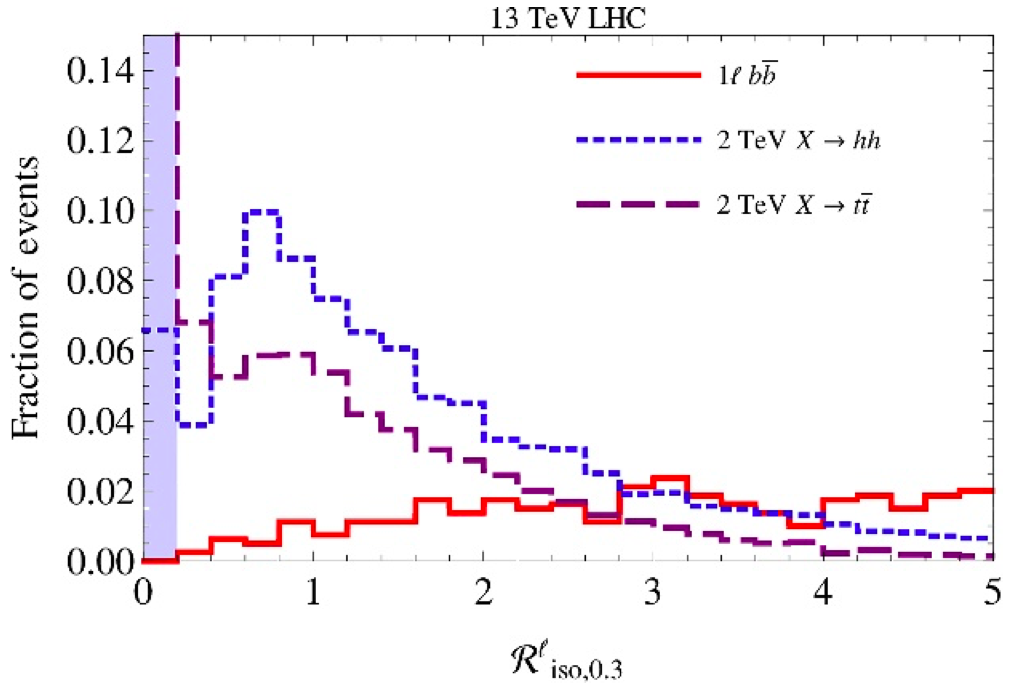
\includegraphics[width=0.6\textwidth]{figures/RelIso0_3.png}
    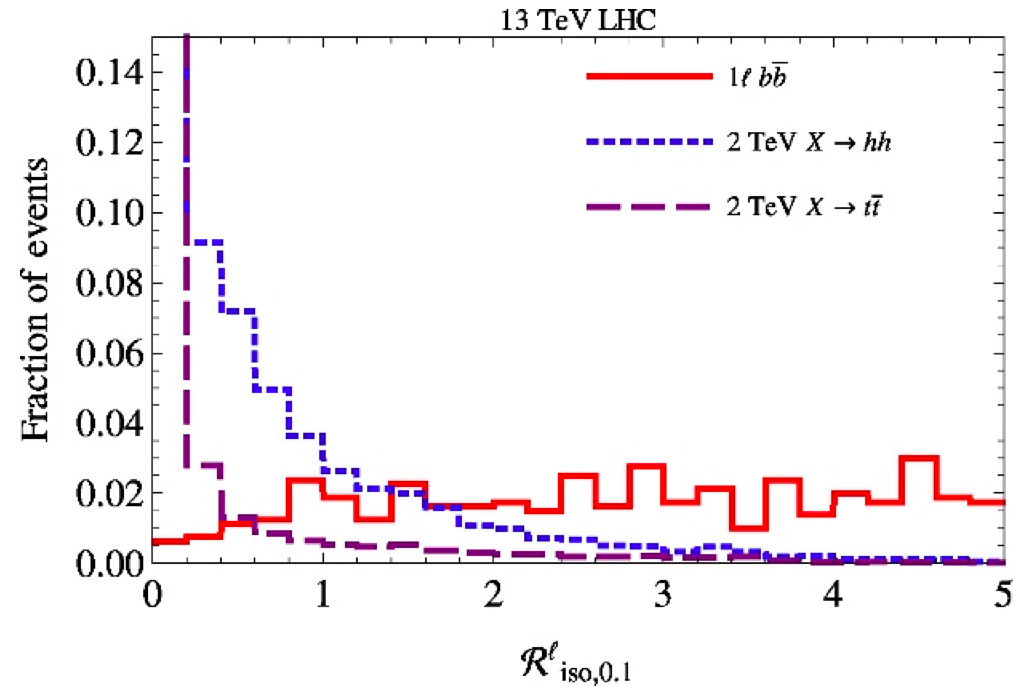
\includegraphics[width=0.6\textwidth]{figures/RelIso0_1.png}
    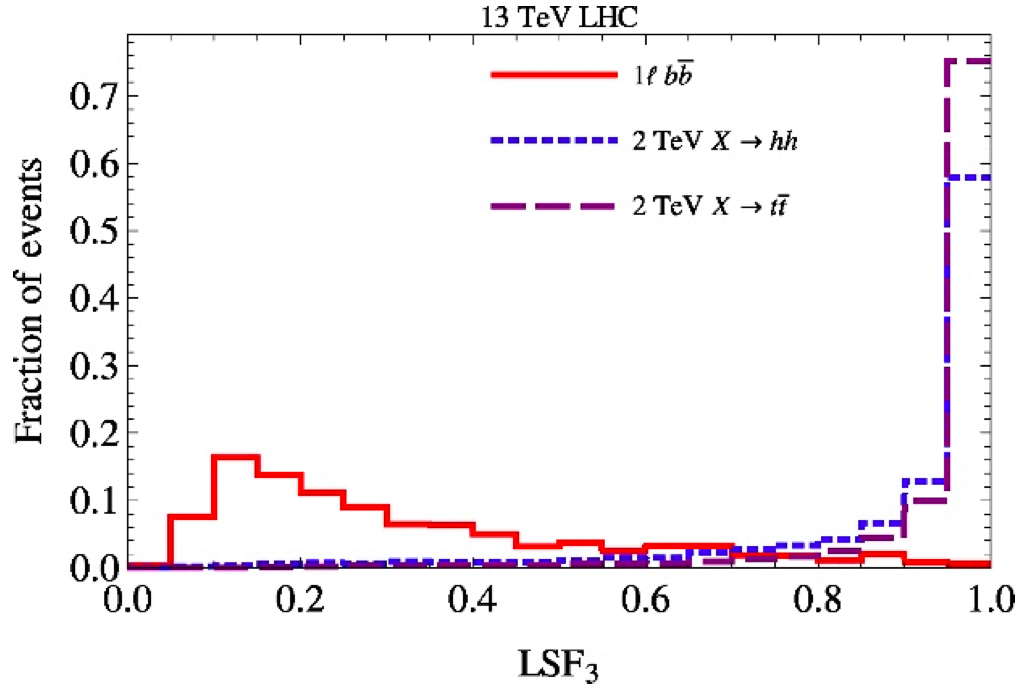
\includegraphics[width=0.6\textwidth]{figures/LSF_paper_plot.png}
    \caption[
        %short caption
        LSF performance compared to relative isolation
    ]    
    {
        From top to bottom, these plots show the performance of a relative isolation cut of 0.3, 0.1, and LSF_{3}.  Each shows the behavior for a semi-leptonic \ensuremath{b\bar{b}} and a theoretical \ensuremath{\SI{2}{\TeV}} object decaying to two Higgs or a \ensuremath{t\bar{t}} pair.
    }
    \label{fig:LSFvRelIso}

\end{figure}

\subsubsection{Soft Drop Mass}

At hadron colliders, there is a significant need to understand the source of interactions in the detector.  At \CMS  and others, multiple events with potentially many products each interact and are recorded simultaneously in a bunch crossing.  Disentangling the constituents of a jet as being from the key hard process of interest, or simply a QCD interaction in the event is important. This process is called ``jet grooming''. Soft drop mass is a tune-able way to remove softer, less energetic contributions to a jet.  The idea being that softer contributions more likely come from background interactions. Other jet grooming techniques exist, but \CMS uses soft drop mass.

While the jet algorithm used at \CMS and in this analysis, is anti-\ensuremath{k_t}, the jet constituents are re-clustered with the Cambridge-Aachen (C/A) algorithm which creates a pair based clustering scheme with angular ordering. More information on the C/A and anti-\ensuremath{k_t} algorithm can be found here \cite{AK_jets}. The C/A clustering is brought to where there are just two subjets, we can label them as \ensuremath{j_1} and \ensuremath{j_2}.  These are then compared with
\begin{equation}
    \label{eq:SDmass}
    \frac{min\left(p_{T1},p_{T2}\right)}
    {p_{T1}+p_{T2}}
    >
    z_{cut}\left( \frac{\Delta R_{12}}{R_{0}} \right) ^ {\beta}
\end{equation}

The behaviour is then tune-able with two variables: \ensuremath{z_{cut}} and \ensuremath{\beta}, depending on the desired response.

If this condition is true, then jet \ensuremath{j} is the final soft-drop jet.  If this is not the case, \ensuremath{j} is redefined to be the subjet with larger \pt and the procedure continues.  In the case that \ensuremath{j} is unable to be declustered j is either removed from consideration or left as the final soft-drop jet.  At \CMS typically \ensuremath{\beta = 0} and \ensuremath{z_{cut} = 0.1}.  Having \ensuremath{\beta = 0} essentially removes dependence on separation, and instead drops subjets if they have less than \ensuremath{10\%} of the total of transverse momentum of the pair.  Then angular associating of the subjets comes from the C/A algorithm which creates the pairing tree.  More detail on the C/A  and \akalgorithm algorithm can be found here \cite{AK_jets}.  The soft drop mass procedure is proposed in this paper \cite{SoftDrop}.

\section{Right-Handed Neutrino Jets}
\label{sec:RNjets}
While LRS models do not give any suggestions for the \NR and \WR mass relationship, searches where the \NR is lighter, but of the same order of magnitude as the \WR have been performed. It is however, just as possible that the mass of the \NR be significantly lighter than the \WR mass \ensuremath{m_{\NR} / m_{\WR} \leq 0.1}. In this situation the neutrinos will be produced with large transverse momentum, and the lepton and two quarks from the \NR decay will be collimated in the lab frame. 
\begin{figure}[!tp]
    \centering
    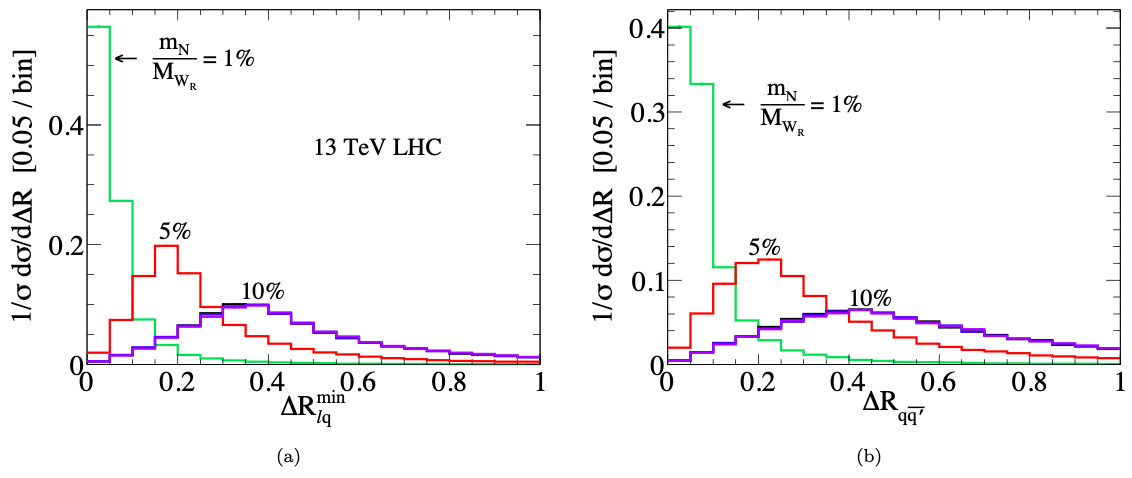
\includegraphics[width=\textwidth]{figures/nrjet_paper_plot.png}
    \caption[
        %short caption
        Angular separation of boosted \NR decay products
    ]    
    {
        Minimum angular separation of the lepton and a quark from \NR decays (a) and the separation of the two quarks in the \NR decay (b) are shown. Three different mass ratios of the \NR and \WR are shown in each. As this analysis clusters jets of size $\Delta R = 0.8$, virtually all of these \NR decays would have their quarks and lepton found within the jet\cite{nrjets}.
    }
    \label{fig:nsubjettiness}

\end{figure}
A detailed discussion of \NR ``jets'' can be found in \cite{nrjets}.

%\section{Continuing Searches}

%A section to briefly detail some of the more interesting ``state-of-the-art'' boosted physics analyses: Higgs to BB, B2G, etc.